\usetikzlibrary{arrows.meta}

\begin{figure}[htb]
	\begin{center}
		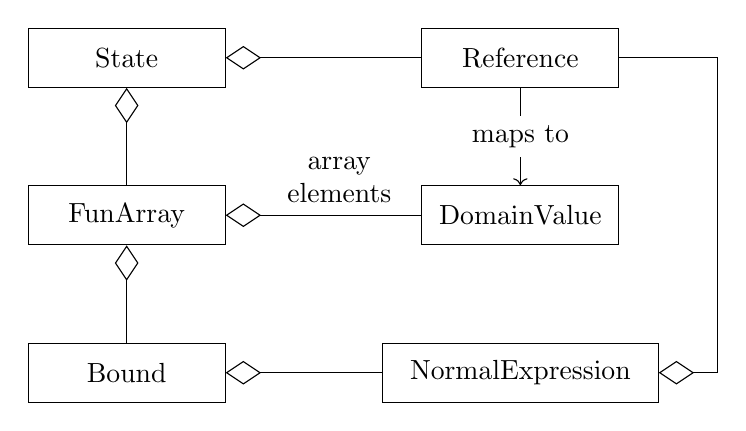
\begin{tikzpicture}
         
 
         \node [rectangle, draw, minimum width=2.5cm, minimum height=0.75cm] (bound)       at (0,0)    {Bound};
         \node [rectangle, draw, minimum width=2.5cm, minimum height=0.75cm] (array)       at (0,2)    {FunArray};
         \node [rectangle, draw, minimum width=2.5cm, minimum height=0.75cm] (state)       at (0,4)    {State};
         
         \node [rectangle, draw, minimum width=3.5cm, minimum height=0.75cm] (expression)  at (5,0)    {NormalExpression};
         \node [rectangle, draw, minimum width=2.5cm, minimum height=0.75cm] (value)       at (5,2)    {DomainValue};
         \node [rectangle, draw, minimum width=2.5cm, minimum height=0.75cm] (reference)   at (5,4)    {Reference};

         \draw [{Diamond[open, length=4.5mm, width=3mm]}-] (state) -- (array);
         \draw [{Diamond[open, length=4.5mm, width=3mm]}-] (array) -- (bound);
         \draw [{Diamond[open, length=4.5mm, width=3mm]}-] (bound) -- (expression);
         \draw [{Diamond[open, length=4.5mm, width=3mm]}-] (state) -- (reference);
         
         \draw [{Diamond[open, length=4.5mm, width=3mm]}-] (array) -- node[align=center, yshift=4.5mm, xshift=2mm]{array\\elements} (value);
         \draw [->](reference) -- node[fill=white!5]{maps to} (value);
         \draw [{Diamond[open, length=4.5mm, width=3mm]}-](expression) -- (7.5,0) -- (7.5,4) --(reference);
        
        \end{tikzpicture}
        \caption{A simplified UML-like diagram showcasing the architecture of a program state.}\label{fig:uml_analyser}
	\end{center}
\end{figure}